\documentclass[11pt,a4paper]{jarticle}
\usepackage[dvipdfmx]{graphicx}
\usepackage{url}

\renewcommand{\baselinestretch}{1.05} 
\marginparwidth=0cm
\topmargin=-1cm
\headheight=0.3cm
\headsep=0.7cm
\oddsidemargin=0cm
\evensidemargin=0cm
%\textwidth=43zw
\textwidth=15.92cm
%\textheight=43.3\baselineskip
\baselineskip = 0.5744cm
\textheight=43\baselineskip

\itemsep=0.05\baselineskip
\parsep=0pt
\topsep=0.01\baselineskip
\partopsep=0pt
\listparindent=0zw

%% header and footer
\usepackage{fancyhdr}
\pagestyle{fancy}
\lhead{2014年度 春学期授業}
\chead{インタラクティブ・アート実習}
\rhead{担当教員: 松下 光範}
\cfoot{\thepage}
\renewcommand{\headrulewidth}{0pt}
\renewcommand{\footrulewidth}{0pt}

\usepackage{ascmac}
\usepackage{listings,jlisting}
\usepackage{color}
\definecolor{OliveGreen}{cmyk}{0.64,0,0.95,0.40}
\definecolor{colFunc}{rgb}{1,0.07,0.54}
\definecolor{CadetBlue}{cmyk}{0.62,0.57,0.23,0}
\definecolor{Brown}{cmyk}{0,0.81,1,0.60}
\definecolor{colID}{rgb}{0.63,0.44,0}
\definecolor{rulesepcolor}{gray}{0.666}
\lstset{
  language=Java,%プログラミング言語によって変える。
  basicstyle={\ttfamily\small},
  keywordstyle={\color{OliveGreen}},
  %[2][3]はプログラミング言語によってあったり、なかったり
  keywordstyle={[2]\color{colFunc}},
  keywordstyle={[3]\color{CadetBlue}},%
  commentstyle={\color{Brown}},
  %identifierstyle={\color{colID}},
  stringstyle=\color{blue},
  tabsize=2,
  %frame=trBL,
  %numbers=left,
  numberstyle={\ttfamily\small},
  breaklines=true,%折り返し
  %backgroundcolor={\color[gray]{.95}},
  framexleftmargin=0mm,
  frame=shadowbox,
  rulesepcolor=\color{rulesepcolor},
  captionpos=b
}


%%%%%%%%%%%%%%%%%%%%%%%%%%%%%%%%%%%%%%%%%%%%%%%%%%%%%%%%%%%%%%%%
\begin{document}

% title
\section*{\LARGE{第1講 基本的なプログラミングと電子回路の作成}}
Processing を使って絵を書く。
基本的な子電回路を組む。

%%%%%%%%%%%%%%%%%%%%%%%%%%%%%%%%%%%%%%%%%%%%%%%%%%%%%%%%%%%%%%%%


\section{下準備}
\subsection*{ノート PC の準備}
本実習では、各個人に 1 台のノート PC を割り当てます。
次回の授業からは開始までに、あらかじめロッカー内から自分が使用するノート PC を取り出して準備を行なってください。
授業終了時には、ノート PC を収められていた箱に収納し、ロッカー内の指定位置まで返却してください。

このノート PC は、\textbf{他の実習授業でも使用します}ので、まず最初に各個人のアカウントを作成します。
\textbf{授業内の作業は、各個人アカウントで行うようにしてください}。
指示にしたがって、共有アカウントでログインし、個人用アカウントの作成、パスワードの設定を行なってください。

\subsection*{実習で用いる部品}
\begin{figure}[h!]
 \begin{minipage}{0.5\columnwidth}
  \centering
  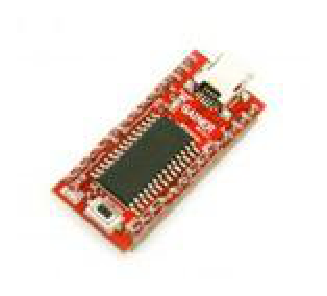
\includegraphics[height=0.4\columnwidth]{img/arduino.eps}
  \caption{Arduino UNO}
 \end{minipage}
 \begin{minipage}{0.5\columnwidth}
  \centering
  
\includegraphics[height=0.4\columnwidth]{img/breadboard.eps}
  \caption{ブレッドボード}
 \end{minipage}
\end{figure}

\begin{figure}[h!]
 \begin{minipage}{0.5\columnwidth}
  \centering
  \includegraphics[height=0.4\columnwidth]{img/jumpwire.eps}
  \caption{ジャンプワイヤ}
 \end{minipage}
 \begin{minipage}{0.5\columnwidth}
  \centering
  \includegraphics[height=0.4\columnwidth]{img/jumpwire.eps}
  \caption{【図を差し替える】抵抗、スイッチ、センサ etc.}
 \end{minipage}
\end{figure}

\begin{itembox}{注意!}
 Arduino などの電子部品は壊れやすいので取り扱いに注意してください。
 \begin{itemize}
  \item 静電気 (Arduino が壊れてしまいます)
  \item 電子部品のピンは曲がりやすいので無理に差し込まないように注意! (壊れます)
  \item PC に刺したまま配線をいじらない (最悪、PC ごと壊れます・・・)
 \end{itemize}
\end{itembox}


\section{Processing の基礎}
本実習では Processing\footnote{\url{http://processing.org}} というプログラミング言語を用います。
Processingは、Java を単純化し、グラフィック機能に特化した言語です。

\begin{figure}[h]
 \centering
 \includegraphics[width=0.5\columnwidth]{img/processing_ide.eps}
 \caption{Processing の IDE (統合開発環境)}
\end{figure}

\subsection*{基本的な図形を描く}

\begin{itemize}
 \item \textbf{四角形を書く}: rect(x, y, w, h);

       x = x座標、
       y = y座標、
       w = 四角形の幅、
       h = 四角形の高さ

 \item \textbf{円を書く}: ellipse(x, y, w, h);
       
       x = x座標、
       y = y座標、
       w = 円の幅、
       h = 円の高さ

 \item \textbf{線を書く}: line(x1, y1, x2, y2);
       
       x1 = 始点のx座標、
       y1 = 始点のy座標、
       x2 = 終点のx座標、
       y2 = 終点のy座標

 % \item \textbf{三角形を書く}: triangle(x1, y1, x2, y2, x3, y3);

\end{itemize}

\subsubsection*{サンプルコード}

\begin{figure}[h!]
 \begin{minipage}{0.65\columnwidth}
  \begin{lstlisting}
   // 画面サイズを幅300px、高さ200pxに設定
   size(300, 200);

   rect(10, 30, 120, 100); // 四角形を描く

   line(10, 10, 290, 190); // 線を描く

   ellipse(200, 120, 100, 150); // 円を描く
  \end{lstlisting}  
 \end{minipage}
 \begin{minipage}{0.35\columnwidth}
  \centering
  \includegraphics[width=0.5\columnwidth]{img/circuit01.eps}
  % \includegraphics[width=0.5\columnwidth]{img/sample_code_01.eps}
 \end{minipage}
\end{figure}


\subsection*{図形の色を変える}

\begin{itemize}
 \item \textbf{図形に色をつける}: fill(r, g, b);

       r, g, b をそれぞれ 256 段階で指定
       % r = Red の値
       % g = Green の値
       % b = Blue の値

       % \begin{itembox}{Tips}
       % 	fill(r, g, b) のように RBG それぞれの値で色を指定する方法の他に、	
       % 	fill(grey) のように黒から白の 256 段階で指定する方法があります。
       
       % 	例えば、fill(0) は黒、fill(255) は白になります。
       % 	また、fill(0, 0, 0) と fill(0) は同じ意味です。
       % \end{itembox}

       % gray = 0 -> 黒、
       % gray = 255 -> 白
       % value = r, g, b に同じ値を代入する

 \item \textbf{色を消す}: noFill();
       
 \item \textbf{縁取り線に色をつける}: stroke(r, g, b);
       
       % stroke(value);

 \item \textbf{縁取り線の幅を調節する}: strokeWeight(weight);
       
       weight = 線の太さ

 \item \textbf{縁取り線を消す}: noStroke();

 \item \textbf{ウィンドウの背景色を指定する}: background(r, g, b);

       % background(grey);

\end{itemize}

\subsubsection*{サンプルコード}

\begin{figure}[h!]
 \begin{minipage}{0.65\columnwidth}
  \begin{lstlisting}
   size(300, 200);

   // 背景を黒に
   // background(0, 0, 0); と同じ意味
   background(0); 

   fill(255, 0, 0); // 四角形を赤に
   rect(10, 30, 120, 100);

   stroke(0, 255, 0); // 線を緑に
   line(10, 10, 290, 190);

   strokeWeight(3); // 線の太さを3pxに
   fill(0, 0, 255); // 円を緑に
   ellipse(200, 120, 100, 150);
  \end{lstlisting}
 \end{minipage}
 \begin{minipage}{0.35\columnwidth}
  \centering
  \includegraphics[width=0.5\columnwidth]{img/circuit01.eps}
  % \includegraphics[width=0.5\columnwidth]{img/sample_code_01.eps}
 \end{minipage}
\end{figure}



\subsection*{アニメーションを作る}
Processing では、プログラムを実行時に setup 関数が 1 度実行され (初期化) 、その後 draw関数 が繰り返される (ループ処理)。

\begin{lstlisting}
 void setup(){
   // 初期化の処理をここに書く
   // プログラム開始時に1度だけ実行される
   size(200, 200); // ウィンドウサイズの指定
 }

 void draw(){
   // 繰り返したい処理をここに書く
   // setup()が実行された後にプログラムが終了するまで繰り返される
   line
 }
\end{lstlisting}


\begin{itemize}
 \item \textbf{マウスの座標を取得する}: mouseX, mouseY
 \item \textbf{hoge}
\end{itemize}


% \begin{itembox}{Tips}
%  メニューバーの「Help → Reference」でインターネットブラウザが起動し、より詳しい説明が確認できますので、そちらも参考にしてください。
%  ただし、英語表記です。
%  Processing にはあらかじめサンプルコード (お手本になるプログラム) が、たくさん用意されているので、それを動かしてみてどんなことができるかを見ておくのも良いかもしれません。
%  サンプルコードは、メニューバーの「File → Example」から見ることができます。
% \end{itembox}



\section{電子回路の基礎}

\subsection*{電気、電流、抵抗のおさらい}
よく、電気の流れは水の流れに例えられます。
厳密にいえばさまざまな違いはありますが、その性質を大まかにとらえるには、水の流れに例えて理解するのは有効な方法です。

\subsubsection*{電圧}
% 電圧は 2 点間の高度 (電位) の違いを表す用語です。
% 水は高度の高いところから低いところに向けて流れますが、電気も電位の高いところから低いところに向けて流れます。
% 水の場合には、それぞれの地点の高さを比較するのに、海抜などを基準として用います。
% 電気の場合には、グランド (GND) を基準として比較します。
% 電子回路ではよく「グランドを接続する」ということが行われます。
% これは、基準であるグランドを共通にしないと、回路の部分ごとの電圧の基準が共通にならず、意図した通りに電気が流れてくれないためです。
% 電圧の単位はボルト (V) です。
% 数字が大きければ大きいほど、電圧が高いことを示します。

\subsubsection*{電流}
% 電流は、水の流れが水流であるのと同じように電気の流れです。
% 電流は、電圧の高いところから低いところに向けて流れます。
% 水流も多い場合少ない場合がありますが、電流も多い場合や少ない場合があります。
% 電流の単位はアンペア (A) です。
% 数字が大きければ大きいほど、多くの電気が流れることを意味します。

\subsubsection*{抵抗}
% 水の場合にも、何も障害物がない場合と、くねくね曲がって流れにくくしている場合では、水の流れにく
% さが異なります。
% 同様に、電気の場合にも電流が流れやすい場合と流れにくい場合があります。
% この電流の流れにくさを表すのが抵抗です。
% 抵抗の単位はオーム (Ω) です。
% 数字が大きければ大きいほど、電流が流れにくいことを示します。

\subsubsection*{よく出てくる補助単位}
電圧、電流、抵抗の単位はそれぞれボルト、アンペア、オームですが、実際にはこれに接頭辞がついた補助単位が用いられる場合が多くあります。
以下は、登場する補助単位の例です。
\begin{itemize}
 \item 1,000 倍を表す単位がキロ (例: 10 kΩ)
 \item 1,000,000 倍を表す単位がメガ (例: 1 MΩ)
 \item 1/1,000 を表す単位がミリ (例: 10 mA)
\end{itemize}

\subsubsection*{オームの法則}
電子部品に電圧をかけすぎたり、電流を流しすぎると壊れてしまう。
そのために、電源側に抵抗器を配置し、電流量を調節する必要がある。

オームの法則は、

\begin{equation}
 V (電圧) = I (電流) \times R (抵抗)
\end{equation}

R (抵抗) を求めるために指揮を変形すると、

\begin{equation}
 R = \frac{(電源電圧 - LEDにかかる電圧)}{LEDに流したい電圧}
\end{equation}


\subsection*{スイッチを押したら LED を点灯させる}
Arduino、スイッチ、抵抗、LED を用いて簡単な回路を組む。

% \subsubsection*{電源}
% 電力の供給元
% Gainer mini は 5V と 3.3V を出力することができる。
% 今回は5Vのピンを、電源として用いる。(乾電池1本は 1.5V)

% \subsubsection*{スイッチ}
% 今回用いるのは、押した時だけ通電するスイッチ(タクトスイッチ)
% 内部でつながっている部分の方向に注意!

% \subsubsection*{抵抗器}
% 電流の流れにくさをコントロールする。
% 抵抗で LED に流れる電流を制御することができる。
% オームの法則を用いて抵抗値を算出する。
% 実際には、計算結果にぴったりの抵抗器があるとは限らない。
% その場合、近い値の抵抗器を用いる。

% \subsubsection*{LED}
% 正式名称:Light Emitting Diode(発光ダイオード)
% 電圧をかけると発光するダイオードで、消費電力が小さく寿命が長い。
% 赤色で1.8V、青色で3.6V程度の電圧が必要。
% 極性があるので注意! (電流を流す方向を間違えると壊れます...)
% 足が長いほうがアノード(プラス) 短いほうがカソード(マイナス)

\begin{figure}[h!]
 \centering
 \includegraphics[height=80mm]{img/circuit01.eps}
 \caption{回路図}
\end{figure}

\begin{figure}[h!]
 \begin{minipage}{0.5\columnwidth}
  \centering
  \includegraphics[width=0.8\columnwidth]{img/release_switch.eps}
 \end{minipage}
 \begin{minipage}{0.5\columnwidth}
  \centering
  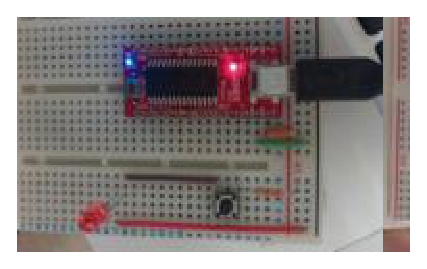
\includegraphics[width=0.8\columnwidth]{img/push_switch.eps}
 \end{minipage}
 \caption{配線例: タクトスイッチを離した状態だと LED が消灯し、押した状態だと LED が点灯する}
\end{figure}

\end{document}
